% Created by tikzDevice version 0.12 on 2018-11-17 19:39:13
% !TEX encoding = UTF-8 Unicode
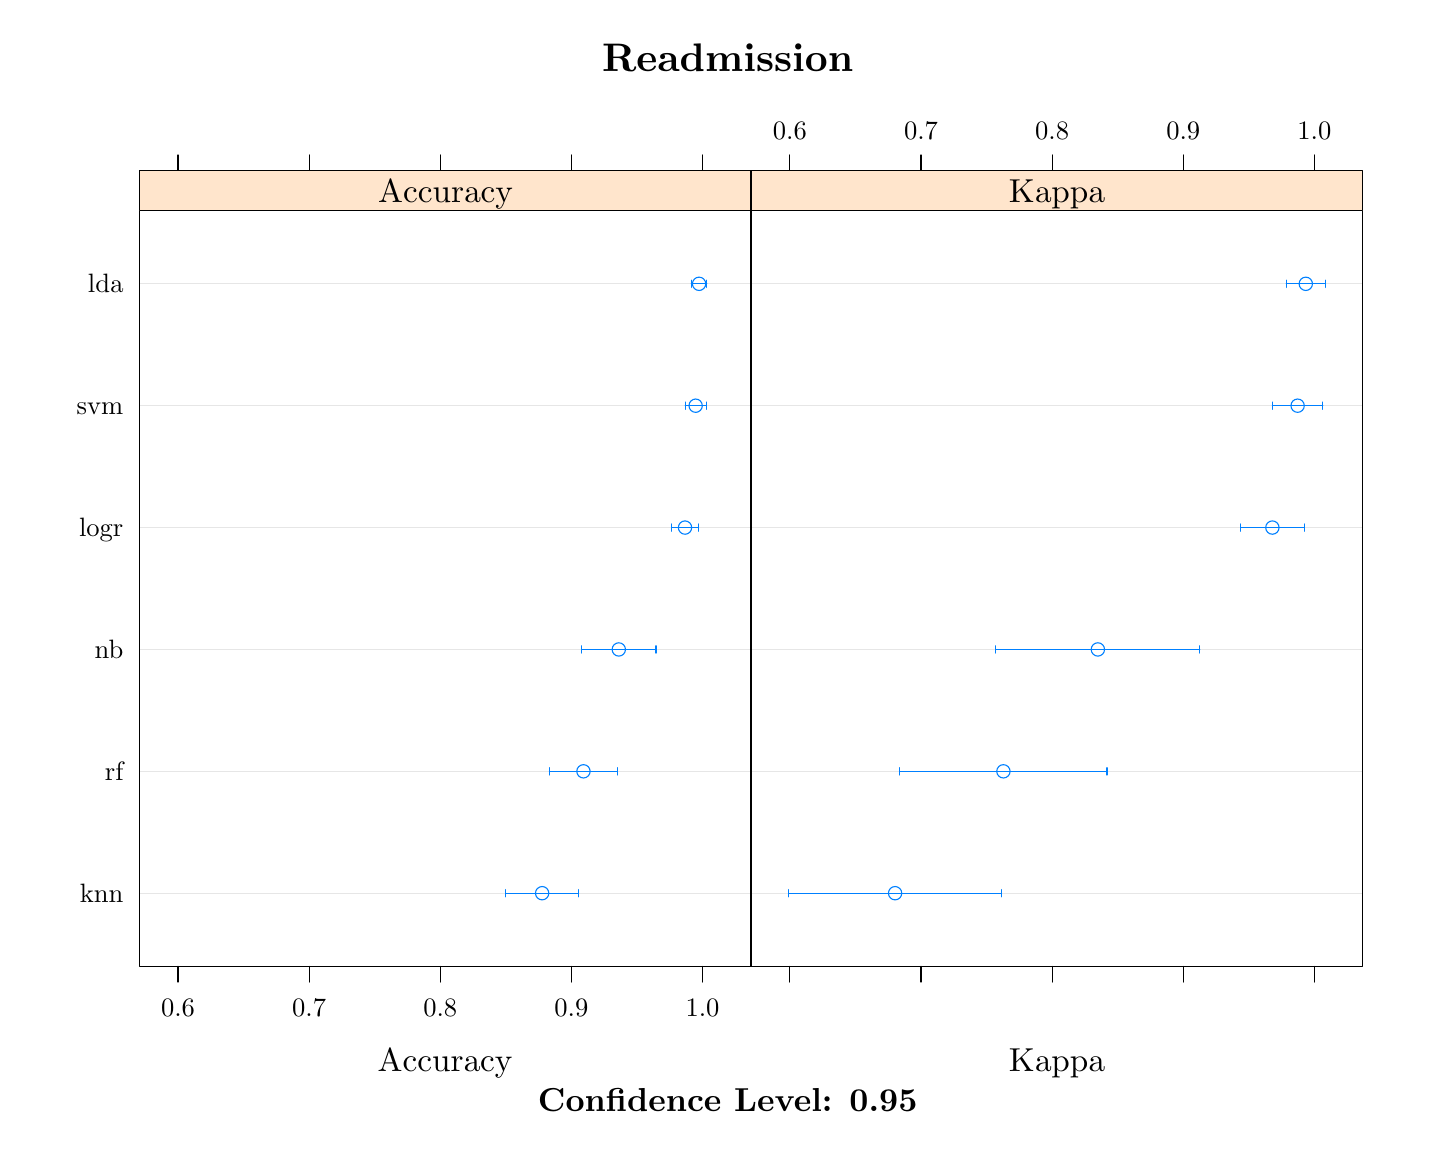
\begin{tikzpicture}[x=1pt,y=1pt]
\definecolor{fillColor}{RGB}{255,255,255}
\path[use as bounding box,fill=fillColor,fill opacity=0.00] (0,0) rectangle (505.89,397.48);
\begin{scope}
\path[clip] (  0.00,  0.00) rectangle (505.89,397.48);

\path[] (  0.00,  0.00) rectangle (505.89,397.48);
\definecolor{drawColor}{RGB}{0,0,0}

\node[text=drawColor,anchor=base,inner sep=0pt, outer sep=0pt, scale=  1.44] at (252.94,381.52) {\bfseries Readmission};
\end{scope}
\begin{scope}
\path[clip] (  0.00,  0.00) rectangle (505.89,397.48);
\definecolor{drawColor}{RGB}{0,0,0}

\node[text=drawColor,anchor=base,inner sep=0pt, outer sep=0pt, scale=  1.20] at (252.94,  6.02) {\bfseries Confidence Level: 0.95};
\end{scope}
\begin{scope}
\path[clip] (  0.00,  0.00) rectangle (505.89,397.48);
\definecolor{drawColor}{RGB}{0,0,0}

\node[text=drawColor,anchor=base,inner sep=0pt, outer sep=0pt, scale=  1.20] at (150.82, 20.33) {Accuracy};

\node[text=drawColor,anchor=base,inner sep=0pt, outer sep=0pt, scale=  1.20] at (371.92, 20.33) {Kappa};
\end{scope}
\begin{scope}
\path[clip] (  0.00,  0.00) rectangle (505.89,397.48);
\definecolor{drawColor}{RGB}{0,0,0}

\path[draw=drawColor,line width= 0.4pt,line join=round,line cap=round] ( 54.33,345.80) -- ( 54.33,351.49);

\path[draw=drawColor,line width= 0.4pt,line join=round,line cap=round] (101.71,345.80) -- (101.71,351.49);

\path[draw=drawColor,line width= 0.4pt,line join=round,line cap=round] (149.10,345.80) -- (149.10,351.49);

\path[draw=drawColor,line width= 0.4pt,line join=round,line cap=round] (196.48,345.80) -- (196.48,351.49);

\path[draw=drawColor,line width= 0.4pt,line join=round,line cap=round] (243.86,345.80) -- (243.86,351.49);
\end{scope}
\begin{scope}
\path[clip] (  0.00,  0.00) rectangle (505.89,397.48);
\definecolor{drawColor}{RGB}{0,0,0}

\node[text=drawColor,anchor=base east,inner sep=0pt, outer sep=0pt, scale=  0.96] at ( 34.58, 81.41) {knn};

\node[text=drawColor,anchor=base east,inner sep=0pt, outer sep=0pt, scale=  0.96] at ( 34.58,125.45) {rf};

\node[text=drawColor,anchor=base east,inner sep=0pt, outer sep=0pt, scale=  0.96] at ( 34.58,169.49) {nb};

\node[text=drawColor,anchor=base east,inner sep=0pt, outer sep=0pt, scale=  0.96] at ( 34.58,213.53) {logr};

\node[text=drawColor,anchor=base east,inner sep=0pt, outer sep=0pt, scale=  0.96] at ( 34.58,257.57) {svm};

\node[text=drawColor,anchor=base east,inner sep=0pt, outer sep=0pt, scale=  0.96] at ( 34.58,301.61) {lda};
\end{scope}
\begin{scope}
\path[clip] (  0.00,  0.00) rectangle (505.89,397.48);
\definecolor{drawColor}{RGB}{0,0,0}

\path[draw=drawColor,line width= 0.4pt,line join=round,line cap=round] ( 54.33, 58.30) -- ( 54.33, 52.61);

\path[draw=drawColor,line width= 0.4pt,line join=round,line cap=round] (101.71, 58.30) -- (101.71, 52.61);

\path[draw=drawColor,line width= 0.4pt,line join=round,line cap=round] (149.10, 58.30) -- (149.10, 52.61);

\path[draw=drawColor,line width= 0.4pt,line join=round,line cap=round] (196.48, 58.30) -- (196.48, 52.61);

\path[draw=drawColor,line width= 0.4pt,line join=round,line cap=round] (243.86, 58.30) -- (243.86, 52.61);

\node[text=drawColor,anchor=base,inner sep=0pt, outer sep=0pt, scale=  0.96] at ( 54.33, 40.30) {0.6};

\node[text=drawColor,anchor=base,inner sep=0pt, outer sep=0pt, scale=  0.96] at (101.71, 40.30) {0.7};

\node[text=drawColor,anchor=base,inner sep=0pt, outer sep=0pt, scale=  0.96] at (149.10, 40.30) {0.8};

\node[text=drawColor,anchor=base,inner sep=0pt, outer sep=0pt, scale=  0.96] at (196.48, 40.30) {0.9};

\node[text=drawColor,anchor=base,inner sep=0pt, outer sep=0pt, scale=  0.96] at (243.86, 40.30) {1.0};
\end{scope}
\begin{scope}
\path[clip] ( 40.28, 58.30) rectangle (261.37,331.34);
\definecolor{drawColor}{RGB}{230,230,230}

\path[draw=drawColor,line width= 0.4pt,line join=round,line cap=round] ( 40.28, 84.72) -- (261.37, 84.72);

\path[draw=drawColor,line width= 0.4pt,line join=round,line cap=round] ( 40.28,128.76) -- (261.37,128.76);

\path[draw=drawColor,line width= 0.4pt,line join=round,line cap=round] ( 40.28,172.80) -- (261.37,172.80);

\path[draw=drawColor,line width= 0.4pt,line join=round,line cap=round] ( 40.28,216.84) -- (261.37,216.84);

\path[draw=drawColor,line width= 0.4pt,line join=round,line cap=round] ( 40.28,260.88) -- (261.37,260.88);

\path[draw=drawColor,line width= 0.4pt,line join=round,line cap=round] ( 40.28,304.92) -- (261.37,304.92);
\definecolor{drawColor}{RGB}{0,128,255}

\path[draw=drawColor,line width= 0.4pt,line join=round,line cap=round] (185.90, 84.72) circle (  2.41);

\path[draw=drawColor,line width= 0.4pt,line join=round,line cap=round] (200.83,128.76) circle (  2.41);

\path[draw=drawColor,line width= 0.4pt,line join=round,line cap=round] (213.60,172.80) circle (  2.41);

\path[draw=drawColor,line width= 0.4pt,line join=round,line cap=round] (237.53,216.84) circle (  2.41);

\path[draw=drawColor,line width= 0.4pt,line join=round,line cap=round] (241.37,260.88) circle (  2.41);

\path[draw=drawColor,line width= 0.4pt,line join=round,line cap=round] (242.61,304.92) circle (  2.41);

\path[draw=drawColor,line width= 0.4pt,line join=round,line cap=round] (172.76, 84.72) -- (199.03, 84.72);

\path[draw=drawColor,line width= 0.4pt,line join=round,line cap=round] (188.57,128.76) -- (213.08,128.76);

\path[draw=drawColor,line width= 0.4pt,line join=round,line cap=round] (200.17,172.80) -- (227.03,172.80);

\path[draw=drawColor,line width= 0.4pt,line join=round,line cap=round] (232.75,216.84) -- (242.30,216.84);

\path[draw=drawColor,line width= 0.4pt,line join=round,line cap=round] (237.61,260.88) -- (245.13,260.88);

\path[draw=drawColor,line width= 0.4pt,line join=round,line cap=round] (239.79,304.92) -- (245.44,304.92);

\path[draw=drawColor,line width= 0.4pt,line join=round,line cap=round] (172.76, 86.04) -- (172.76, 83.40);

\path[draw=drawColor,line width= 0.4pt,line join=round,line cap=round] (188.57,130.08) -- (188.57,127.44);

\path[draw=drawColor,line width= 0.4pt,line join=round,line cap=round] (200.17,174.12) -- (200.17,171.48);

\path[draw=drawColor,line width= 0.4pt,line join=round,line cap=round] (232.75,218.16) -- (232.75,215.52);

\path[draw=drawColor,line width= 0.4pt,line join=round,line cap=round] (237.61,262.20) -- (237.61,259.56);

\path[draw=drawColor,line width= 0.4pt,line join=round,line cap=round] (239.79,306.24) -- (239.79,303.60);

\path[draw=drawColor,line width= 0.4pt,line join=round,line cap=round] (199.03, 86.04) -- (199.03, 83.40);

\path[draw=drawColor,line width= 0.4pt,line join=round,line cap=round] (213.08,130.08) -- (213.08,127.44);

\path[draw=drawColor,line width= 0.4pt,line join=round,line cap=round] (227.03,174.12) -- (227.03,171.48);

\path[draw=drawColor,line width= 0.4pt,line join=round,line cap=round] (242.30,218.16) -- (242.30,215.52);

\path[draw=drawColor,line width= 0.4pt,line join=round,line cap=round] (245.13,262.20) -- (245.13,259.56);

\path[draw=drawColor,line width= 0.4pt,line join=round,line cap=round] (245.44,306.24) -- (245.44,303.60);
\end{scope}
\begin{scope}
\path[clip] (  0.00,  0.00) rectangle (505.89,397.48);
\definecolor{drawColor}{RGB}{0,0,0}

\path[draw=drawColor,line width= 0.4pt,line join=round,line cap=round] ( 40.28, 58.30) rectangle (261.37,331.34);
\end{scope}
\begin{scope}
\path[clip] ( 40.28,331.34) rectangle (261.37,345.80);
\definecolor{drawColor}{RGB}{255,229,204}
\definecolor{fillColor}{RGB}{255,229,204}

\path[draw=drawColor,line width= 0.4pt,line join=round,line cap=round,fill=fillColor] ( 40.28,331.34) rectangle (261.37,345.80);
\definecolor{drawColor}{RGB}{0,0,0}

\node[text=drawColor,anchor=base west,inner sep=0pt, outer sep=0pt, scale=  1.20] at (126.65,334.44) {Accuracy};
\end{scope}
\begin{scope}
\path[clip] (  0.00,  0.00) rectangle (505.89,397.48);
\definecolor{drawColor}{RGB}{0,0,0}

\path[draw=drawColor,line width= 0.4pt,line join=round,line cap=round] ( 40.28,331.34) rectangle (261.37,345.80);
\end{scope}
\begin{scope}
\path[clip] (  0.00,  0.00) rectangle (505.89,397.48);
\definecolor{drawColor}{RGB}{0,0,0}

\path[draw=drawColor,line width= 0.4pt,line join=round,line cap=round] (275.42,345.80) -- (275.42,351.49);

\path[draw=drawColor,line width= 0.4pt,line join=round,line cap=round] (322.81,345.80) -- (322.81,351.49);

\path[draw=drawColor,line width= 0.4pt,line join=round,line cap=round] (370.19,345.80) -- (370.19,351.49);

\path[draw=drawColor,line width= 0.4pt,line join=round,line cap=round] (417.57,345.80) -- (417.57,351.49);

\path[draw=drawColor,line width= 0.4pt,line join=round,line cap=round] (464.96,345.80) -- (464.96,351.49);

\node[text=drawColor,anchor=base,inner sep=0pt, outer sep=0pt, scale=  0.96] at (275.42,357.18) {0.6};

\node[text=drawColor,anchor=base,inner sep=0pt, outer sep=0pt, scale=  0.96] at (322.81,357.18) {0.7};

\node[text=drawColor,anchor=base,inner sep=0pt, outer sep=0pt, scale=  0.96] at (370.19,357.18) {0.8};

\node[text=drawColor,anchor=base,inner sep=0pt, outer sep=0pt, scale=  0.96] at (417.57,357.18) {0.9};

\node[text=drawColor,anchor=base,inner sep=0pt, outer sep=0pt, scale=  0.96] at (464.96,357.18) {1.0};
\end{scope}
\begin{scope}
\path[clip] (  0.00,  0.00) rectangle (505.89,397.48);
\definecolor{drawColor}{RGB}{0,0,0}

\path[draw=drawColor,line width= 0.4pt,line join=round,line cap=round] (275.42, 58.30) -- (275.42, 52.61);

\path[draw=drawColor,line width= 0.4pt,line join=round,line cap=round] (322.81, 58.30) -- (322.81, 52.61);

\path[draw=drawColor,line width= 0.4pt,line join=round,line cap=round] (370.19, 58.30) -- (370.19, 52.61);

\path[draw=drawColor,line width= 0.4pt,line join=round,line cap=round] (417.57, 58.30) -- (417.57, 52.61);

\path[draw=drawColor,line width= 0.4pt,line join=round,line cap=round] (464.96, 58.30) -- (464.96, 52.61);
\end{scope}
\begin{scope}
\path[clip] (261.37, 58.30) rectangle (482.46,331.34);
\definecolor{drawColor}{RGB}{230,230,230}

\path[draw=drawColor,line width= 0.4pt,line join=round,line cap=round] (261.37, 84.72) -- (482.46, 84.72);

\path[draw=drawColor,line width= 0.4pt,line join=round,line cap=round] (261.37,128.76) -- (482.46,128.76);

\path[draw=drawColor,line width= 0.4pt,line join=round,line cap=round] (261.37,172.80) -- (482.46,172.80);

\path[draw=drawColor,line width= 0.4pt,line join=round,line cap=round] (261.37,216.84) -- (482.46,216.84);

\path[draw=drawColor,line width= 0.4pt,line join=round,line cap=round] (261.37,260.88) -- (482.46,260.88);

\path[draw=drawColor,line width= 0.4pt,line join=round,line cap=round] (261.37,304.92) -- (482.46,304.92);
\definecolor{drawColor}{RGB}{0,128,255}

\path[draw=drawColor,line width= 0.4pt,line join=round,line cap=round] (313.44, 84.72) circle (  2.41);

\path[draw=drawColor,line width= 0.4pt,line join=round,line cap=round] (352.58,128.76) circle (  2.41);

\path[draw=drawColor,line width= 0.4pt,line join=round,line cap=round] (386.71,172.80) circle (  2.41);

\path[draw=drawColor,line width= 0.4pt,line join=round,line cap=round] (449.77,216.84) circle (  2.41);

\path[draw=drawColor,line width= 0.4pt,line join=round,line cap=round] (458.89,260.88) circle (  2.41);

\path[draw=drawColor,line width= 0.4pt,line join=round,line cap=round] (461.84,304.92) circle (  2.41);

\path[draw=drawColor,line width= 0.4pt,line join=round,line cap=round] (274.95, 84.72) -- (351.93, 84.72);

\path[draw=drawColor,line width= 0.4pt,line join=round,line cap=round] (315.14,128.76) -- (390.02,128.76);

\path[draw=drawColor,line width= 0.4pt,line join=round,line cap=round] (349.86,172.80) -- (423.57,172.80);

\path[draw=drawColor,line width= 0.4pt,line join=round,line cap=round] (438.31,216.84) -- (461.23,216.84);

\path[draw=drawColor,line width= 0.4pt,line join=round,line cap=round] (449.74,260.88) -- (468.04,260.88);

\path[draw=drawColor,line width= 0.4pt,line join=round,line cap=round] (454.79,304.92) -- (468.89,304.92);

\path[draw=drawColor,line width= 0.4pt,line join=round,line cap=round] (274.95, 86.04) -- (274.95, 83.40);

\path[draw=drawColor,line width= 0.4pt,line join=round,line cap=round] (315.14,130.08) -- (315.14,127.44);

\path[draw=drawColor,line width= 0.4pt,line join=round,line cap=round] (349.86,174.12) -- (349.86,171.48);

\path[draw=drawColor,line width= 0.4pt,line join=round,line cap=round] (438.31,218.16) -- (438.31,215.52);

\path[draw=drawColor,line width= 0.4pt,line join=round,line cap=round] (449.74,262.20) -- (449.74,259.56);

\path[draw=drawColor,line width= 0.4pt,line join=round,line cap=round] (454.79,306.24) -- (454.79,303.60);

\path[draw=drawColor,line width= 0.4pt,line join=round,line cap=round] (351.93, 86.04) -- (351.93, 83.40);

\path[draw=drawColor,line width= 0.4pt,line join=round,line cap=round] (390.02,130.08) -- (390.02,127.44);

\path[draw=drawColor,line width= 0.4pt,line join=round,line cap=round] (423.57,174.12) -- (423.57,171.48);

\path[draw=drawColor,line width= 0.4pt,line join=round,line cap=round] (461.23,218.16) -- (461.23,215.52);

\path[draw=drawColor,line width= 0.4pt,line join=round,line cap=round] (468.04,262.20) -- (468.04,259.56);

\path[draw=drawColor,line width= 0.4pt,line join=round,line cap=round] (468.89,306.24) -- (468.89,303.60);
\end{scope}
\begin{scope}
\path[clip] (  0.00,  0.00) rectangle (505.89,397.48);
\definecolor{drawColor}{RGB}{0,0,0}

\path[draw=drawColor,line width= 0.4pt,line join=round,line cap=round] (261.37, 58.30) rectangle (482.46,331.34);
\end{scope}
\begin{scope}
\path[clip] (261.37,331.34) rectangle (482.46,345.80);
\definecolor{drawColor}{RGB}{255,229,204}
\definecolor{fillColor}{RGB}{255,229,204}

\path[draw=drawColor,line width= 0.4pt,line join=round,line cap=round,fill=fillColor] (261.37,331.34) rectangle (482.46,345.80);
\definecolor{drawColor}{RGB}{0,0,0}

\node[text=drawColor,anchor=base west,inner sep=0pt, outer sep=0pt, scale=  1.20] at (354.59,334.44) {Kappa};
\end{scope}
\begin{scope}
\path[clip] (  0.00,  0.00) rectangle (505.89,397.48);
\definecolor{drawColor}{RGB}{0,0,0}

\path[draw=drawColor,line width= 0.4pt,line join=round,line cap=round] (261.37,331.34) rectangle (482.46,345.80);
\end{scope}
\end{tikzpicture}
